\section {EVALUATION} \label{sec:evaluation}

\subsection{Integration techniques}
The pros and cons of all the integration techniques described in Section \ref{sec:integration} are shown in Table \ref{tab:int-technique}. We conclude that REST API was the best integration technique among all the techniques and hence we recommend it to the users of Apache Tika \cite{TikaAndVision}.

\begin{table*}[bt]
	\centering
	\begin{tabularx}{\textwidth}{
			|p{\dimexpr.08\linewidth-2\tabcolsep-1.3333\arrayrulewidth}% column 1
			|p{\dimexpr.08\linewidth-2\tabcolsep-1.3333\arrayrulewidth}% column 1
			|p{\dimexpr.42\linewidth-2\tabcolsep-1.3333\arrayrulewidth}% column 2
			|p{\dimexpr.42\linewidth-2\tabcolsep-1.3333\arrayrulewidth}|% column 3
		} \hline
		
		\textbf{Method} & \textbf{Time} & \textbf{Pros} & \textbf{Cons} \\ \hline
		
		\textbf{CLI} 
		& 3s&
		\tabitem Easy to develop and test \newline
		\tabitem Easy to install dependencies \newline
		\tabitem Isolation of dependencies and concerns
		& \tabitem Additional load on secondary storage to share image data. \newline
		\tabitem An extra process is created and destroyed for each call. \newline
		\tabitem Additional IO for each call since the model file is loaded and unloaded for each process  
		\\ \hline
		
		\textbf{JNI} 
		& N/A
		& \tabitem The most efficient utilization of resources. \newline 
		\tabitem No external IO required since the system is monolithic.
		& 
		\tabitem The JNI native glue code has to be produced for all the platforms. \newline
		\tabitem Utilities like \texttt{protobuf} should also be glued with JNI because they are required for deserializing models\cite{javacpp-240}.
		\\ \hline
		
		\textbf{gRPC}
		& 598ms
		& \tabitem An efficient way for integrating heterogeneous systems. \newline 
		\tabitem The client system is easily portable, the server system can also be easily portable by making use of containerization or virtualization. 
		&  \tabitem The gRPC client depended on specific versions of transitive dependencies such as HTTP Client which conflicts with existing functionality based on older HTTP Clients.
		\\ \hline
		\textbf{REST API}
		& 253ms
		&
		\tabitem An efficient way for integrating heterogeneous systems. \newline 
		\tabitem The technology and practices are popular among developers. \newline 
		\tabitem The underlying HTTP is stable and well documented.
		& \tabitem The bandwidth consumption is higher than gRPC due to the extra HTTP headers. \newline
		\\ \hline
	\end{tabularx}
	\caption{Brief comparison of integration techniques. \textnormal{The numbers in the `Time' column are the time taken per image on a ubuntu 14.04 LTS docker container running on MacBook Pro 2013 model (2.8GhZ Core i7 and SSD storage) for test images of size 1024x768 pixels.}}
	\label{tab:int-technique}
\end{table*}

%%%%%%%% COMMENT BEGIN
\iffalse
\subsubsection{Command Line Invocation (CLI)} \label{sec:eval-cli}
The average time taken to recognize image in this method was 6 seconds.

The pros of Command Line Interface:
\begin{itemize}
	\item Easy to develop and test
	\item Easy to install the requirements
	\item Isolation of dependencies / concerns
\end{itemize}

The cons of this technique:
\begin{itemize}
	\item The image data is shared via secondary storage which puts additional load on the secondary storage.
	\item An independent process is created and destroyed for every parse call.
	\item The ImageNet model is loaded and unloaded for every parse call due to ephemeral nature of processes. The InceptionV3 model used in our experiments is approximately 200MB in size, thus 200MB of additional IO for each parse call.
\end{itemize}

%% 2. JNI
\subsubsection{Java Native Interface (JNI)} \label{sec:eval-jni}

The pros of this method are
\begin{itemize}
	\item The most efficient utilization of resources
	\item No external input-output required as the entire task runs in a single process.
\end{itemize}

The cons of this method are:
\begin{itemize}
	\item The JNI glue code has to be compiled and packaged for all the platforms.
	\item Utilities like \texttt{protobuf} should also be glued with JNI, because they are required for deserializing models\cite{javacpp-240}.
\end{itemize}

%% 3. RPC
\subsubsection{gRPC Remote procedure Call (gRPC)} \label{sec:eval-rpc}

The pros of this method are
\begin{itemize}
	\item An efficient way for integrating heterogeneous systems.
	\item The client system is easily portable, server system can also be easily portable by making use of containerization or virtualization.
\end{itemize}

The cons of this method are:
\begin{itemize}
	\item The gRPC client depended on specific versions of transitive dependencies such as HTTP Client which conflicts with existing functionality based on older HTTP Clients.
\end{itemize}

%% 4. REST
\subsubsection{Representational State Transfer (REST) Application Programming Interface (API)} \label{sec:eval-rest}

The average REST API call was 260 milliseconds when the client and server were in the same host (i.e., the connection via loopback interface).

The pros of this method are
\begin{itemize}
	\item An efficient and popular way for integrating heterogeneous systems.
	\item The technology and practices are popular among developer community.
	\item The underlying HTTP is stable and well documented.
\end{itemize}

The cons of this method are
\begin{itemize}
	\item The performance is slightly lower than gRPC.
	\item Slightly higher bandwidth usage due to additional metadata introduced by HTTP to the packets.
\end{itemize}
\fi  %% COMMENT END

\subsection{Analysis of results}
\begin{figure}[h]
	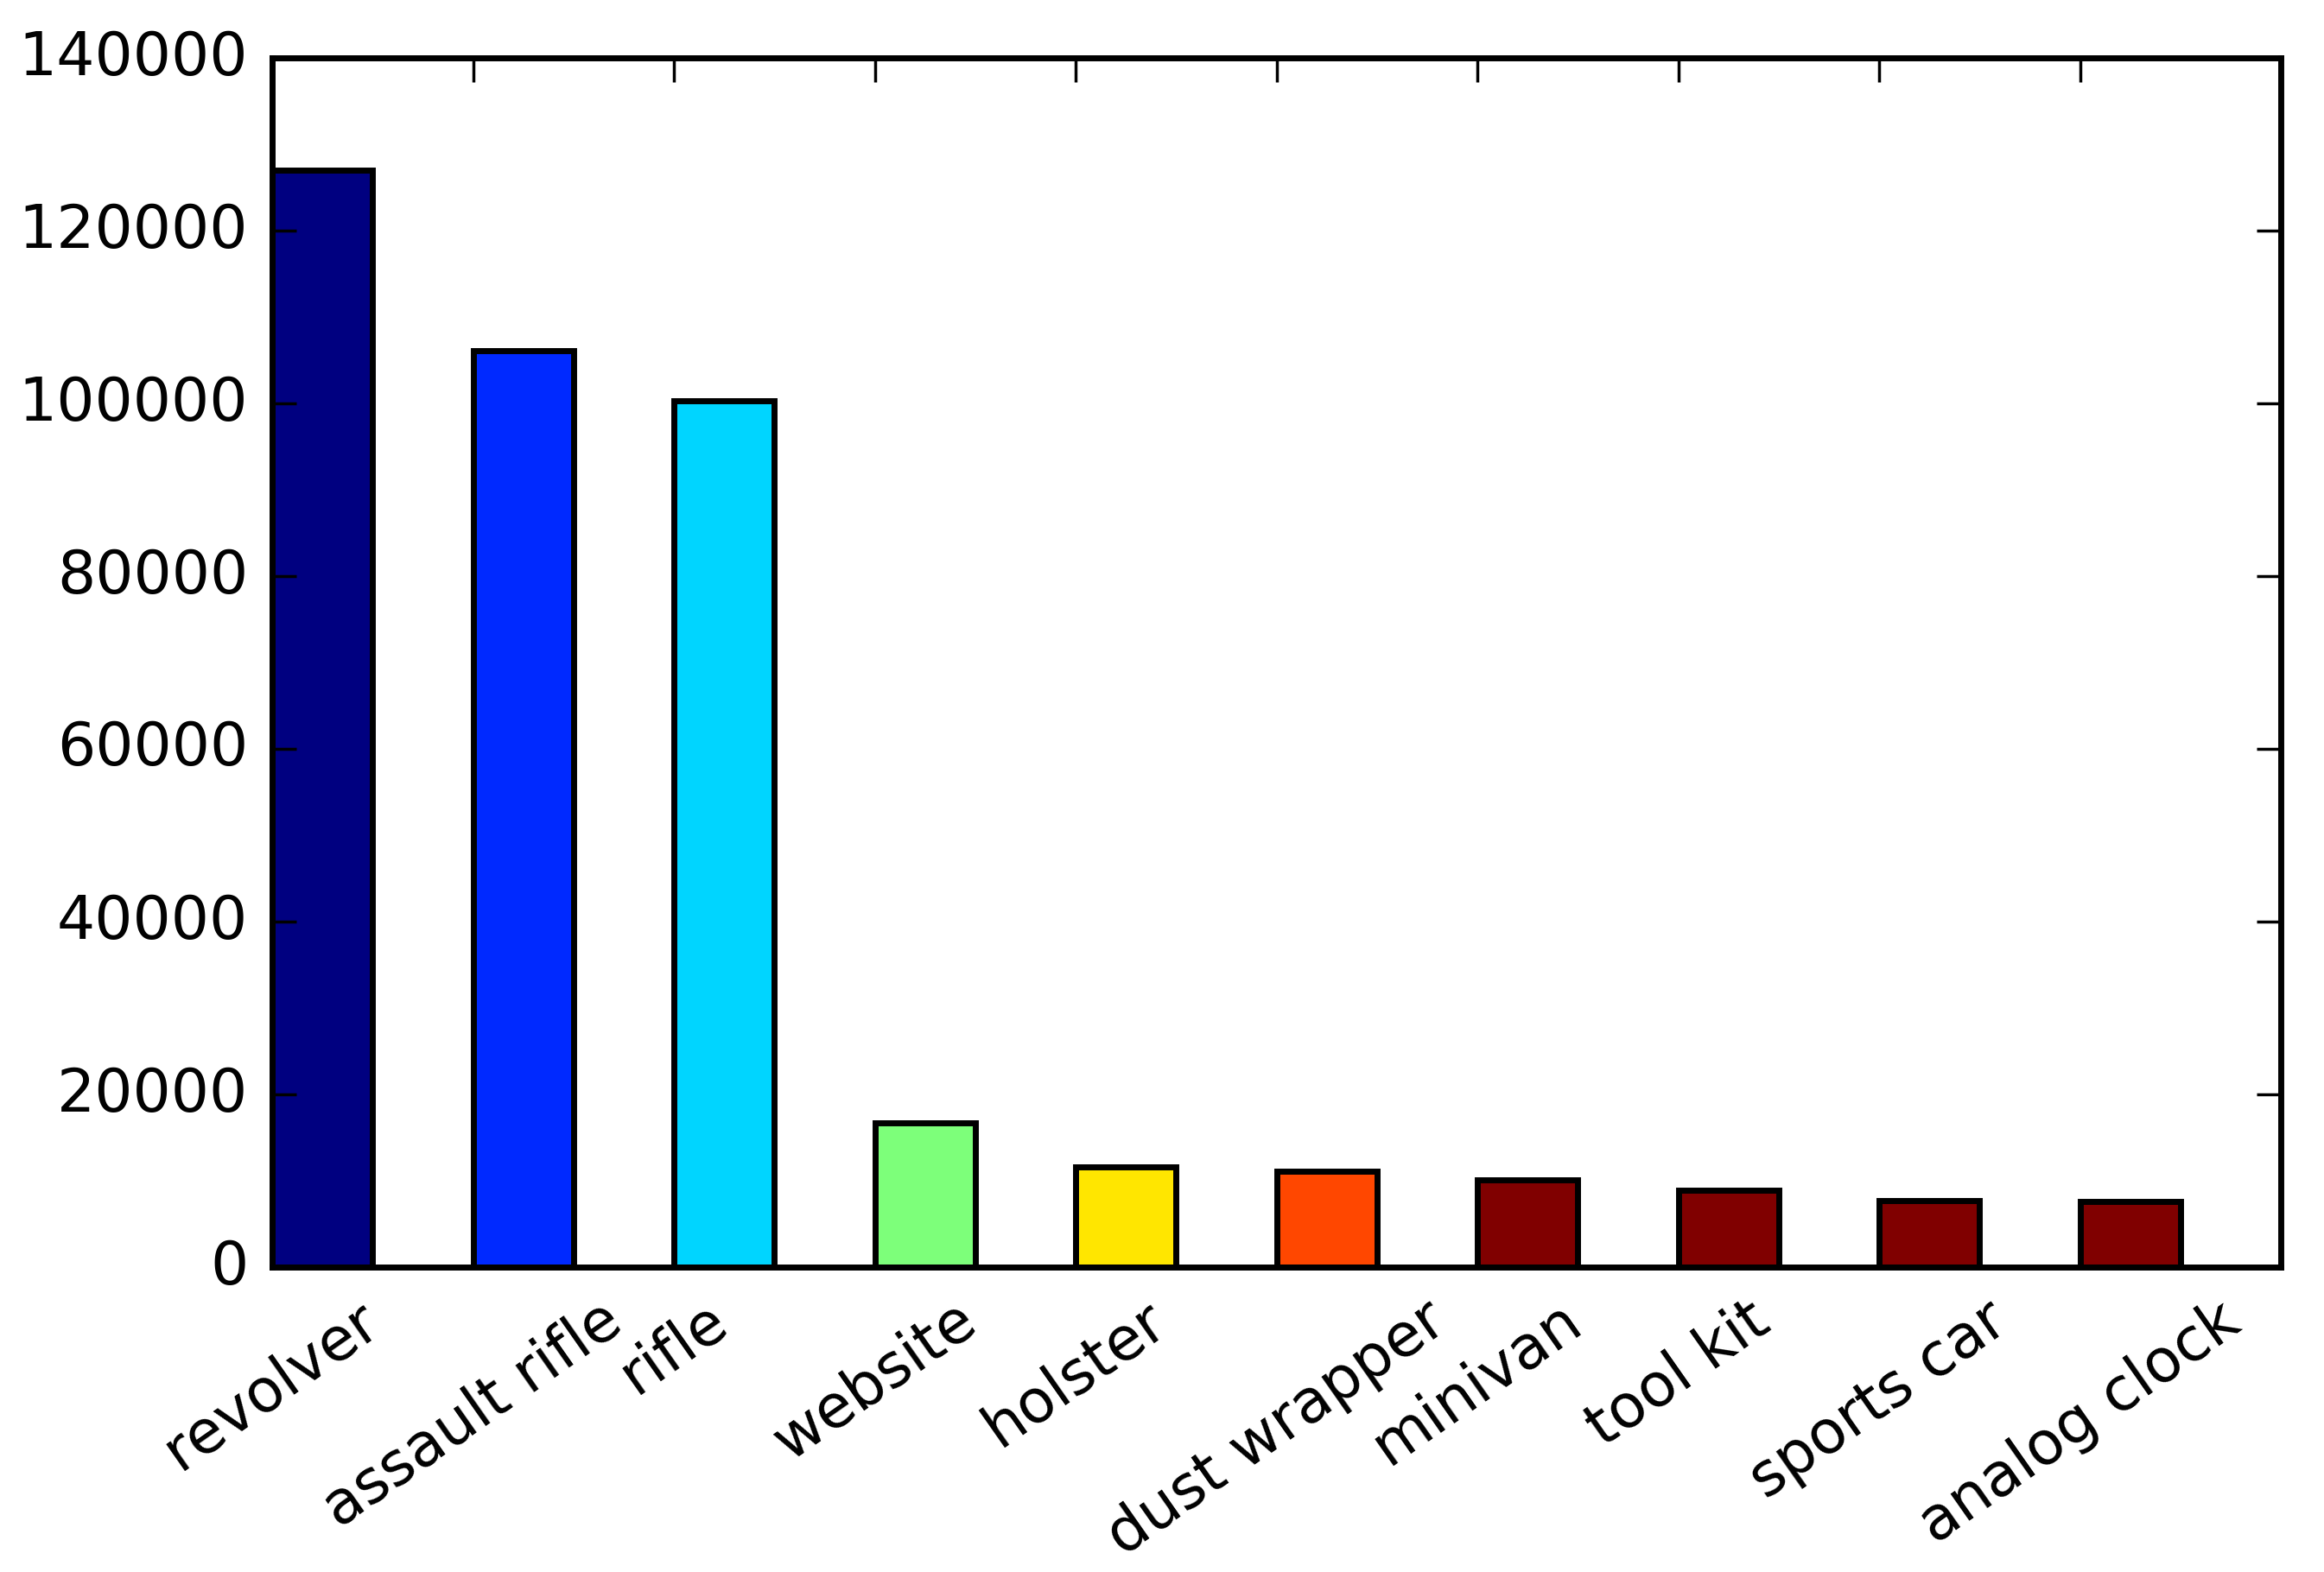
\includegraphics[width=\columnwidth]{top10classes}
	\caption{Top 10 image classes found in the dataset}
	\label{fig:top10ImgClass}
\end{figure}
The image classifier model used in our experiments was Inception-V3 \cite{SzegedyVISW15}. This model has trained on ImageNet 2012 dataset which contains 1000 classes\cite{ILSVRC15}.
The 10 most frequently occurred classes and their frequencies are shown in the Figure \ref{fig:top10ImgClass}. Since the crawlers were focused on retrieving the web pages and linked images that are related to weapons classifieds, the top classes in our dataset were found to be `revolver', and `rifle'

\subsection{Manual cross validation of results}
We cross-validated the predictions by using a subset of human-labeled images. The results are shown in Figure \ref{fig:uk-hack-eval}. The \textit{top k} for $k=1,3,5,7$ considers a prediction as correct if the human annotated label is one among the set of top $k$  predicted labels. We observed that the \textit{top 1} accuracy for the \textit{`revolver'} class is considerably lesser. By manual verification of the labeled images and its prediction errors, we found a pattern that revolvers being the small structure in the images often surrounded by its holders and toolkits; sometimes they placed on top of other items which are also valid classes in ImageNet corpus. The inception model treated the bigger surroundings as the prominent label than the \textit{`revolver'}. In addition, our team in memex program were interested in much granular distinction among the \textit{'rifles'} and \textit{`shotguns'}. Since the ImageNet corpus does not have annotations for sub categories in \textit{`rifles'} and \textit{`shotguns'}, all related truth labels are mapped to \textit{`rifles'} label. 

%//TODO: Describe more if space permits
\begin{figure}[h]
	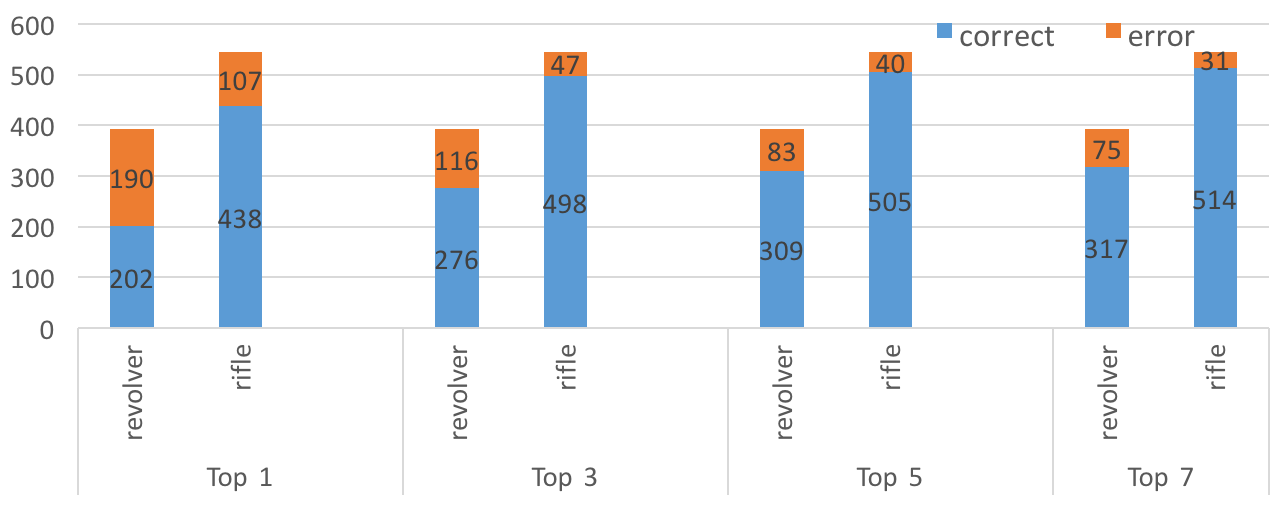
\includegraphics[width=\columnwidth]{uk-hack-evaluation2}
	\caption{Manual cross validation of results for the two weapon types: `revolver' and `rifle'}
	\label{fig:uk-hack-eval}
\end{figure}

